\section{Calcifer}

\begin{minipage}{0.5\textwidth}
\textbf{Name}:Calcifer \\
\textbf{Function}: Main Sophie's helper

\subsection{Internal World}

\textbf{Age \& Gender}: Age not defined. Supposed male \\
\textbf{Values \& Virtues}: Loyalty, friendship\\
\textbf{Personality}: Proud, helpful \\
\textbf{Interests}: Eating to stay alive\\
\textbf{Ethnic Group}: Fire demon

\subsection{External World}
\textbf{Environment}: Howl’s Moving Castle \\
\textbf{Education}: Not defined \\
\textbf{Social \& Cultural Background}: Demons are generally feared and respected by people \\
\textbf{Look \& Feel}: Small yellow and orange flame who becomes big and  blue when he gets enraged or when he has to free his true power\\
\textbf{Job \& Experience}: Fire demon \\

\end{minipage}%
%
\hfill\begin{minipage}{0.4\textwidth}
  \begin{figure}[H]
    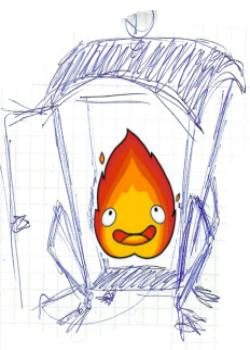
\includegraphics{Images/Characters/lantern}
      % PER ORA HO SCRITTO ELENA COPERCHINI E MESSO LO SCHIZZO DI DAVIDE, DIREI CHE POTREMO CHIEDERE DI DISEGNARCI ANCHE LA LANTERNA
      % MAGARI CON QUALCHE DETTAGLIO PARTICOLARE
    \caption{Calcifer, merge between movie version and sketch of the lantern made by Davide Valentini.}
\end{figure}
\end{minipage}

%% \begin{figure}[H]
%%   {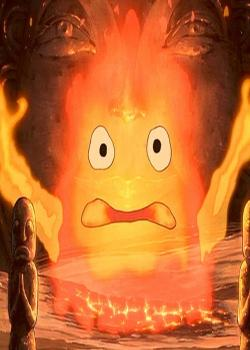
\includegraphics{Images/Characters/calcifer}}		
%%   \qquad%
%%       {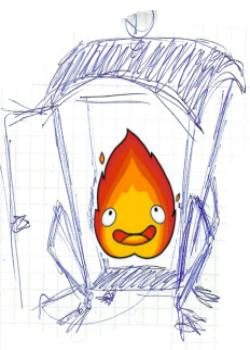
\includegraphics{Images/Characters/lantern}}
%%       % PER ORA HO SCRITTO ELENA COPERCHINI E MESSO LO SCHIZZO DI DAVIDE, DIREI CHE POTREMO CHIEDERE DI DISEGNARCI ANCHE LA LANTERNA
%%       % MAGARI CON QUALCHE DETTAGLIO PARTICOLARE
%%       \caption{Calcifer, movie version on the left. Sketch of the lantern made by Davide Valentini on the right.}
%% \end{figure}

%% \textbf{Name}:Calcifer \\
%% \textbf{Function}: Main Sophie's helper

%% \subsection{Internal World}

%% \textbf{Age \& Gender}: Age not defined. Supposed male \\
%% \textbf{Values \& Virtues}: Loyalty, friendship\\
%% \textbf{Personality}: Proud, helpful \\
%% \textbf{Interests}: Eating to stay alive\\
%% \textbf{Ethnic Group}: Fire demon

%% \subsection{External World}
%% \textbf{Environment}: Howl’s Moving Castle \\
%% \textbf{Education}: Not defined \\
%% \textbf{Social \& Cultural Background}: Demons are generally feared and respected by people \\
%% \textbf{Look \& Feel}: Small yellow and orange flame who becomes big and  blue when he gets enraged or when he has to free his true power\\
%% \textbf{Job \& Experience}: Fire demon \\

\subsubsection*{Relatives \& Relation}
\begin{enumerate}
\item \textbf{Sophie}:She lives with her,he has become one of her best friend and he now really cares for her
\item \textbf{Howl}: He is a long-time friend of him and lives with him in the Moving Castle, evenl after the pact has been broken they are still friends
\item \textbf{Justin}: They are friends, but there is not a stron relationship between them
\item \textbf{Mizar}: He hates her because she is a threat for all of his friends
\item \textbf{Belzel}: He becomes one of his friends after he helps them to find a way to get into the spirits realm
\end{enumerate}

\begin{figure}[H]
  \centering
  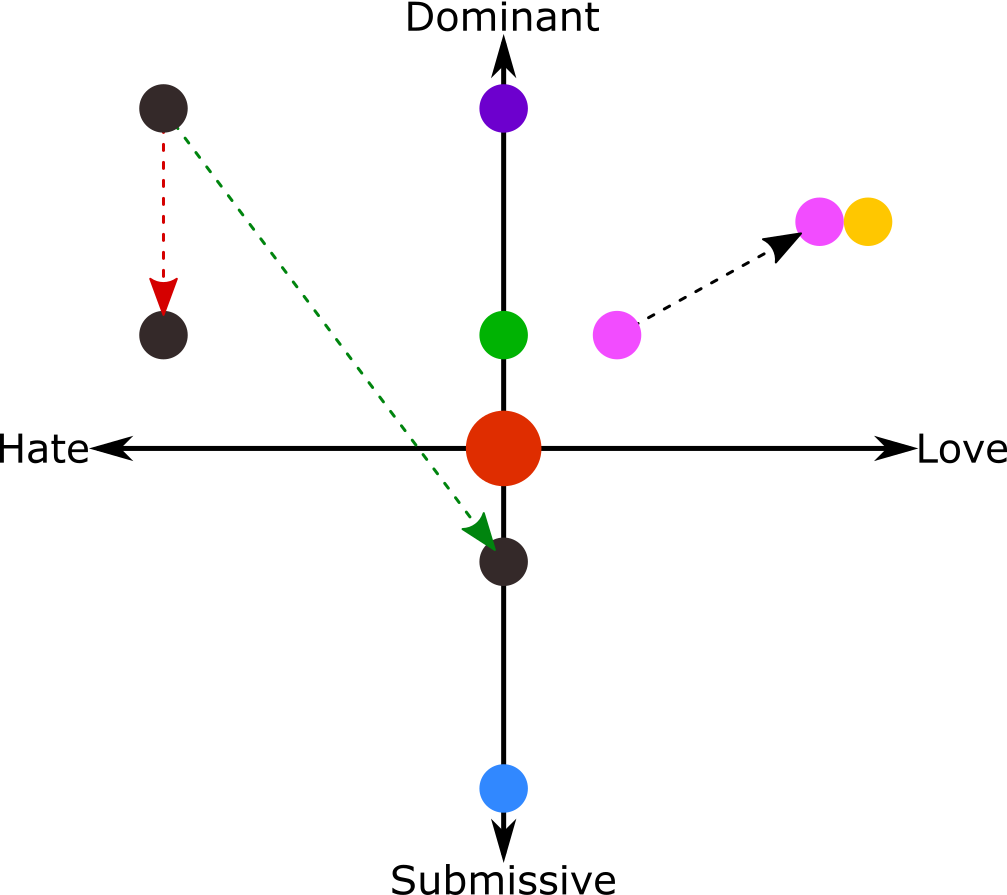
\includegraphics[width=8cm]{Images/Circumplexes/calciferCircumplex}
  \caption{Circumplex of Calcifer}
\end{figure}

\begin{figure}[H]
  \centering
   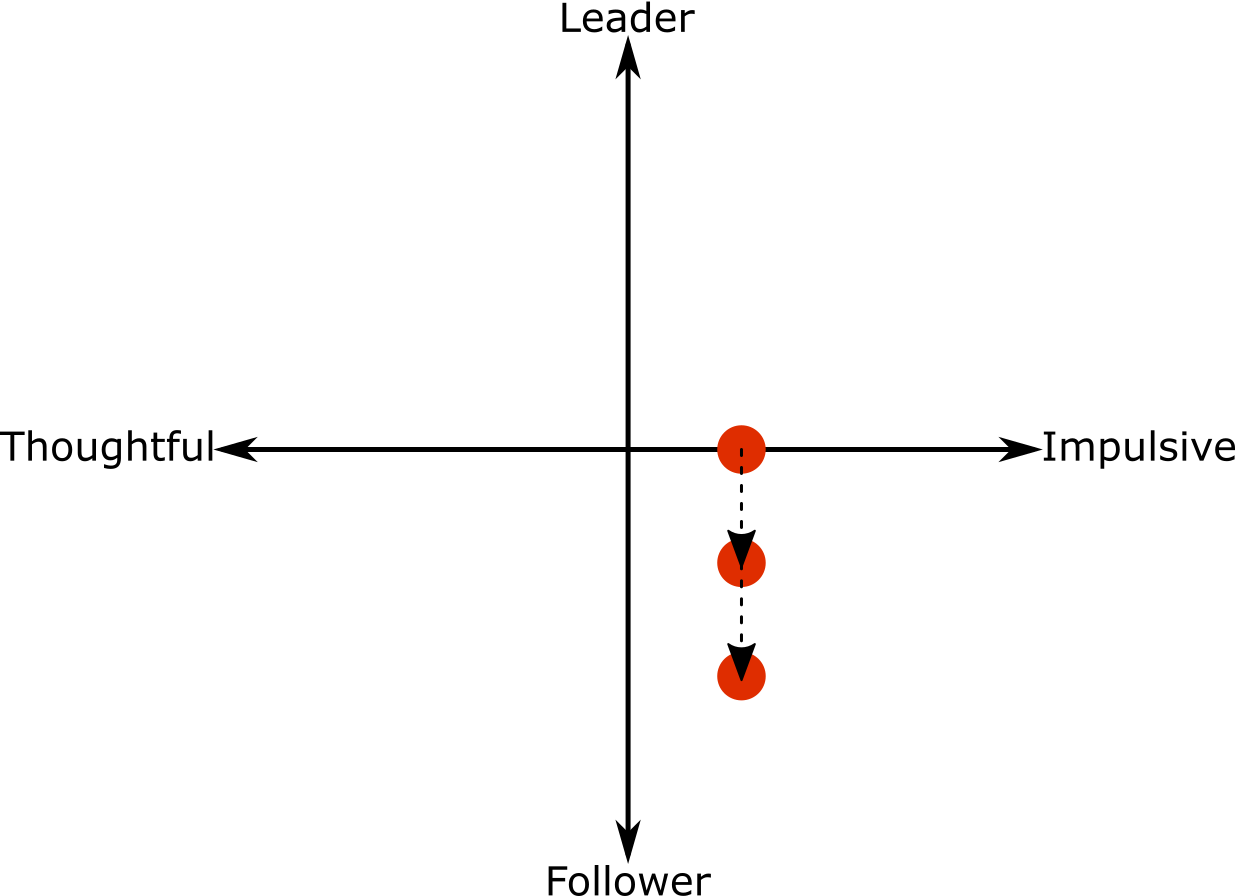
\includegraphics[width=8cm]{Images/Evolutions/calciferEvolution}
  \caption{Evolutions of Calcifer}
\end{figure}

\subsection{Description}
Calcifer always plays the part of a gruff and proud one, but in reality he is a good and loyal friend for both Howl and Sophie, even after the pact was broken. In fact he does whatever he can to help them in every situation and he is one the most willing to go and save Howl.

\subsection{Background story}
Calcifer story has been known since the pact with Howl. His earlier story has been always surrounded by mistery.
